% FIG ch08-08 v1 issue overlay (Chinese).
% Numbered marks sit on the panel each problem belongs to.
% The phrases are listed under the micrograph so they do not cover it.
\tikzset{%
  chviiiissue/.style={%
    circle, draw=BookInk, line width=0.4pt, fill=white, inner sep=0.2pt,%
    minimum size=9pt, font=\sffamily\fontsize{7}{8}\selectfont, text=BookInk%
  },%
  chviiicap/.style={%
    anchor=west, inner xsep=0.4pt, inner ysep=0.5pt,%
    font=\sffamily\fontsize{7}{9}\selectfont, text=BookInk%
  }%
}
\providecommand{\chviiimark}[1]{%
  \tikz[baseline=(n.base)]{\node[chviiiissue] (n) {#1};}%
}
\begin{tikzpicture}
  \node[anchor=south west, inner sep=0pt] (img) at (0,0)
    {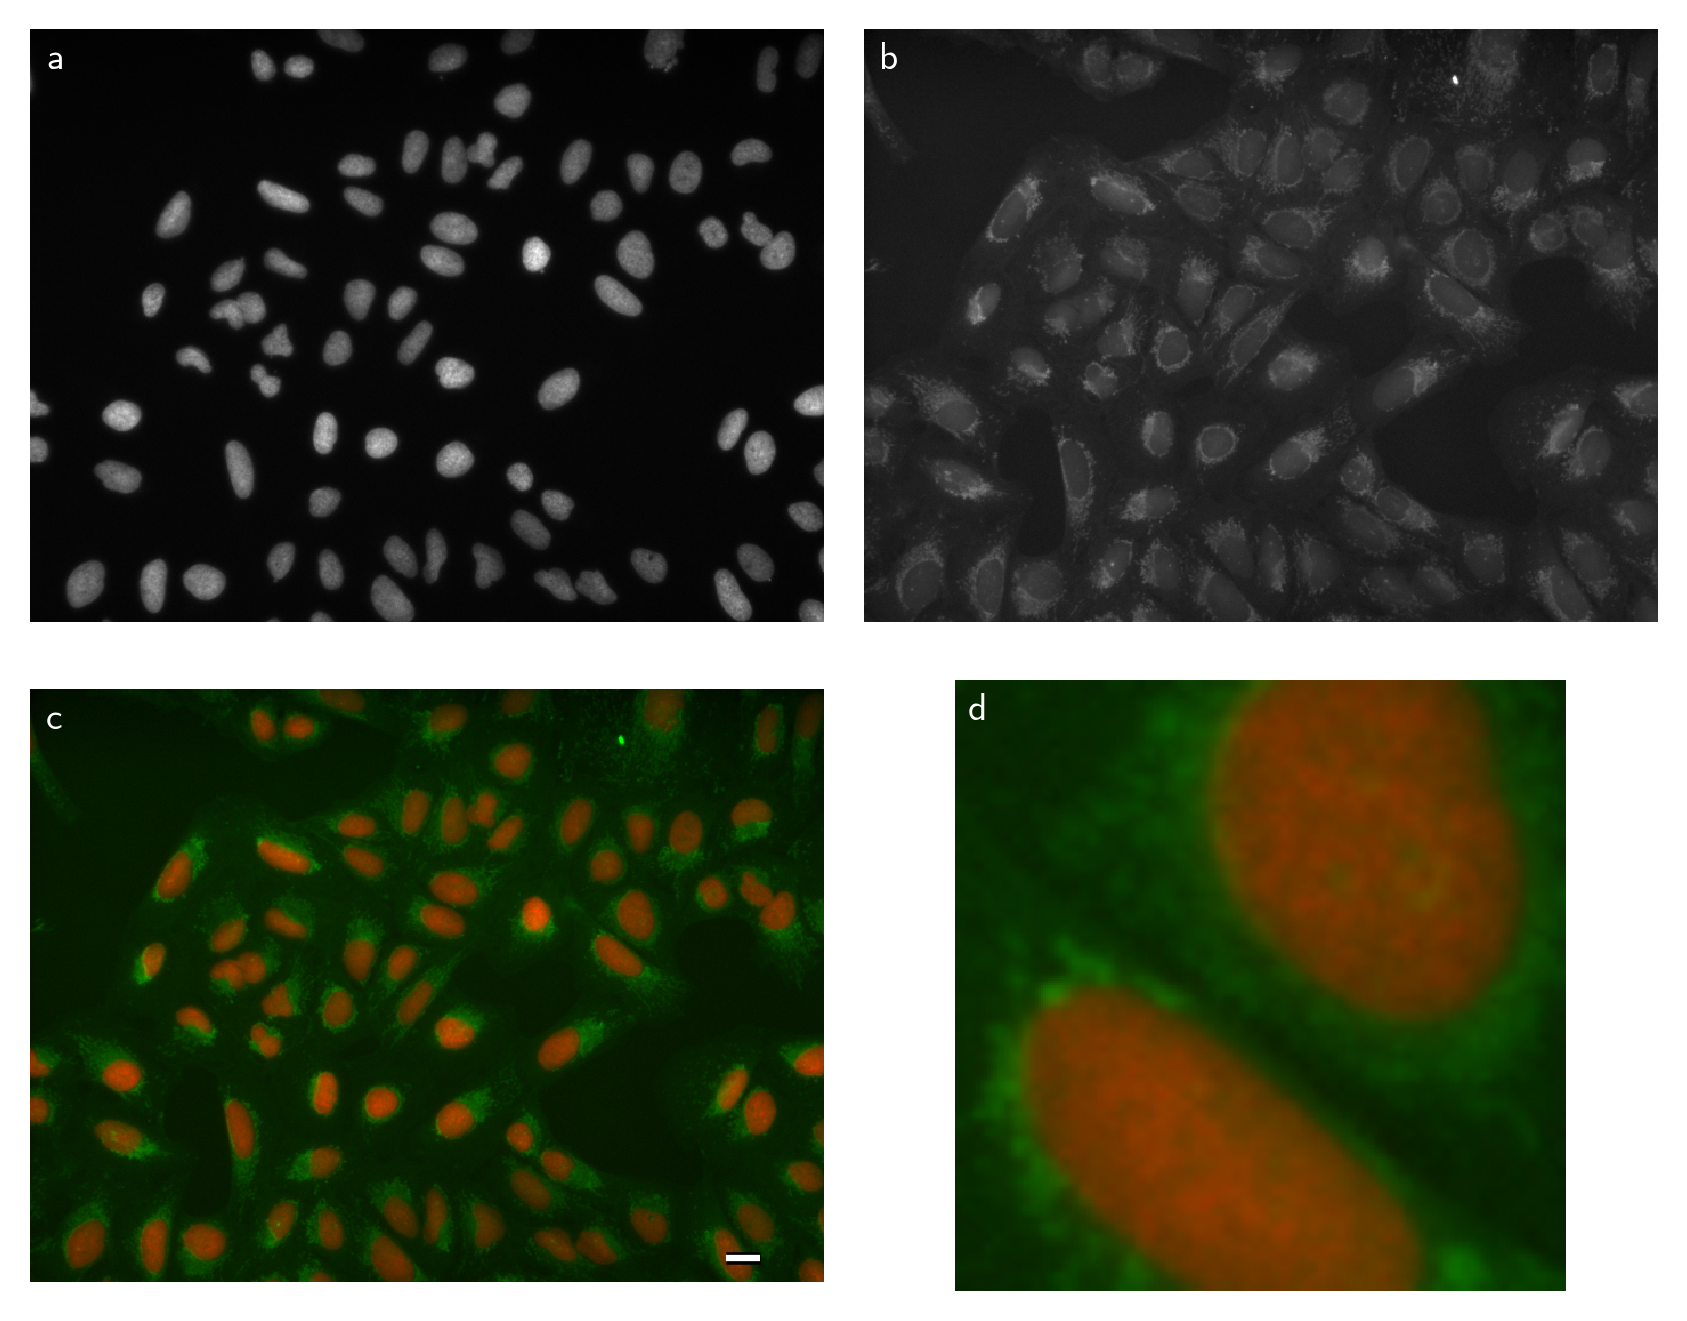
\includegraphics[width=\linewidth]{figures/ch08/ch08-08-case-v1-zh.png}};
  \begin{scope}[x={(img.south east)}, y={(img.north west)}]
    \node[chviiiissue] (m1) at (0.40, 0.92) {1};
    \node[chviiiissue] (m2) at (0.40, 0.45) {2};
    \node[chviiiissue] (m3) at (0.36, 0.09) {3};
    \draw[BookInk, line width=0.35pt] (0.372, 0.078) -- (0.424, 0.056);
    \node[chviiiissue] (m4) at (0.88, 0.12) {4};
    \node[chviiiissue] (m5) at (0.90, 0.92) {5};
  \end{scope}
  \node[chviiicap] (c1) at ([yshift=-1.8mm]img.south west)
    {\chviiimark{1}\enspace 各自自动对比度};
  \node[chviiicap] (c2) at ([yshift=-0.8mm]c1.south west)
    {\chviiimark{2}\enspace 红/绿};
  \node[chviiicap] (c3) at ([yshift=-0.8mm]c2.south west)
    {\chviiimark{3}\enspace 比例尺无依据};
  \node[chviiicap] (c4) at ([yshift=-0.8mm]c3.south west)
    {\chviiimark{4}\enspace 最亮细胞+双三次};
  \node[chviiicap] (c5) at ([yshift=-0.8mm]c4.south west)
    {\chviiimark{5}\enspace 未披露 $\gamma=0.6$};
\end{tikzpicture}
